%----------------------------------------------------------------------------------------
%INTRODUCTION
%----------------------------------------------------------------------------------------

\chapter{Introduction}
Introduction to your report.

% Example of a section 
\section{About the Universe}
Some Information about the Universe in general.

%------------------------------------------------

\section{Literature} % Section

Literature you read to get to know your topic. 
%------------------------------------------------

\section{Description of the galaxy your currently in} % Section

% Example image - change name of picture to your's
\begin{figure}[H] 
\center{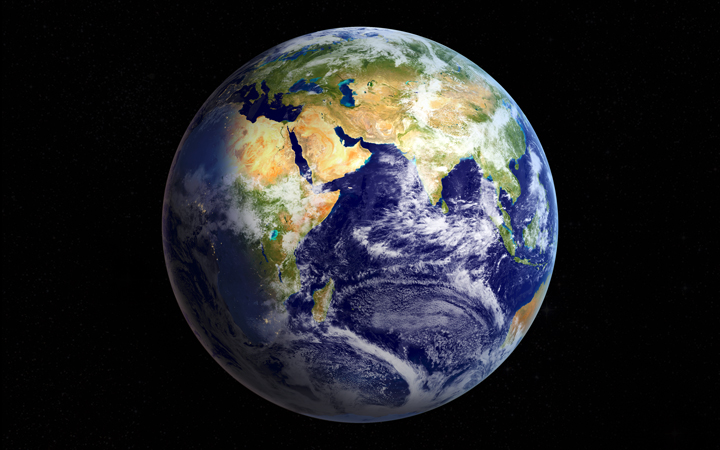
\includegraphics[width=0.5\linewidth]{earth}}
\caption{Planet Earth}
\end{figure}

% Example for a table
\begin{center}
  \begin{tabular}{| m{4.5cm} | m{12cm} |}
    \hline
    \multicolumn{2}{|c|}{Facts} \\ \hline
    Mass & \begin{math} 59736 x 10^{10} kg \end{math} \\ \hline
    Radius (max.) & 6384 km \\ \hline
    Radius (min.) & 6353 km \\ \hline
    \end{tabular}
  \end{center}

% Example of Mini headlines
\textbf{Design}
About Earth's Design.

\textbf{Age}
About Earth's Age

% Example of two images side by side
\textbf{Earth's Neighbors}
\begin{figure}[H]
\centering
\subfloat[Venus]{{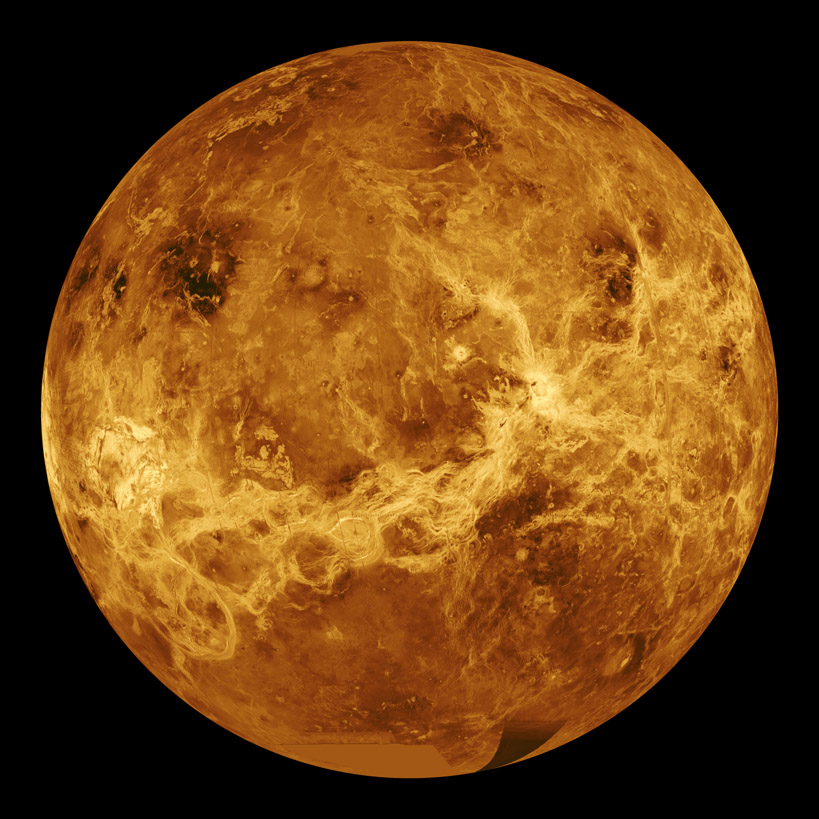
\includegraphics[width=0.25\textwidth]{venus}}}
\qquad
\subfloat[Mars]{{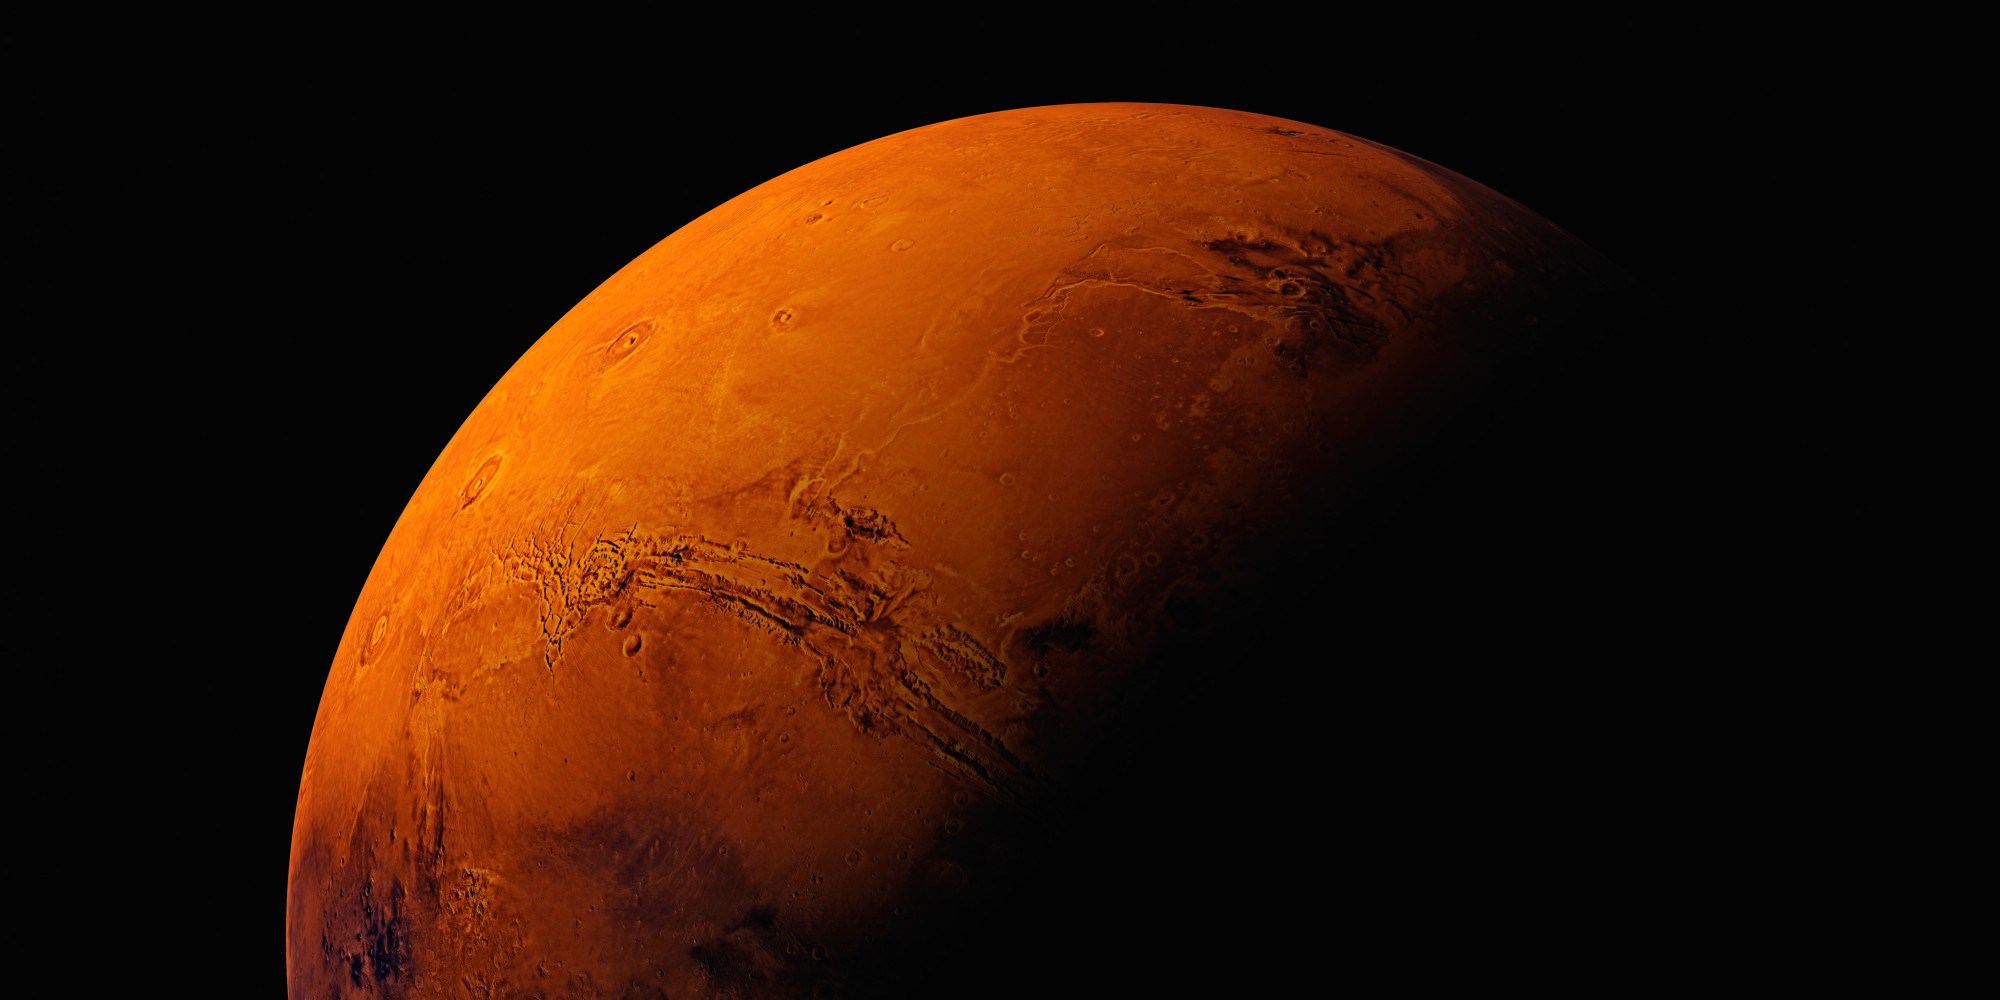
\includegraphics[width=0.25\textwidth]{mars}}}
\end{figure}

% Example of a list with small letters
\begin{enumerate}[label=\alph*)]
  \item{Venus}
is closer to the sun than earth.
  \item{Mars}
    is also known as the red planet.  
\end{enumerate}
%------------------------------------------------


